\documentclass[10pt,twocolumn]{article}

% use the oxycomps style file
\usepackage{oxycomps}

% usage: \fixme[comments describing issue]{text to be fixed}
% define \fixme as not doing anything special
\newcommand{\fixme}[2][]{#2}
% overwrite it so it shows up as red
\renewcommand{\fixme}[2][]{\textcolor{red}{#2}}
% overwrite it again so related text shows as footnotes
%\renewcommand{\fixme}[2][]{\textcolor{red}{#2\footnote{#1}}}

% read references.bib for the bibtex data
\bibliography{references}



% include metadata in the generated pdf file
\pdfinfo{
    /Title (Comps Final Paper)
    /Author (Jacki Jackman)
}
\hypersetup{
    colorlinks=true,
    linkcolor=blue,
    }

% set the title and author information
\title{A Convolutional Neural Network Explorable Explanation: Opening Up Black Box Models Through Interactive Education}
\author{Jacki Jackman}
\affiliation{Occidental College}
\email{jjackman@oxy.edu}

\begin{document}


\maketitle

\section{Introduction and Problem Context}
Neural Networks have now become an integral part of technology; however, a marginally small group of people understand how it functions. Especially with artificial intelligence as one of the highest trending fields within computer science, many students entering the computer science department often aim to work in the field, yet they do not have an understanding of what it entails until junior or senior year of college. Due to the immense amount of coding and mathematical prerequisites generally required to take machine learning courses, there currently exists a high barrier of entry to learn what it entails. 

This project aims to lower the barrier of entry into understanding the functions of neural networks as a gateway into machine learning. It aims to implement the interactive capabilities of webapp UI/UX design to create an explorable explanation as an accessible platform to explain complex technological methods. By looking into how explorable explanations can be applied to teaching black box models, I ultimately hope to better address the issue of opacity in machine learning algorithms. \cite{MLOpacity}

\section{Technical Background}
\subsection{Black Box Models}
Black box models are algorithms that receive data as input and produce an output without explaining the processes it took to produce its prediction. Even designers of the algorithm cannot explain the specific mathematical process occurring within the black box method. Over time a growing belief that black box models produce more accurate results than interpretable models which are constrained to provide users and creators with a better understanding of how predictions are made. This has led to a polarized public discourse in error-prone automation. However, by increasing opacity to black box algorithms, it can encourage a greater level of understanding by the public and responsibility from coders. \cite{BlackBoxModels}

\subsection{Explorable Explanations}
Explorable explanations are "free, browser-based experiences with a high level of interactivity and a more or less even mix between visuals and text that teach facts, concepts and procedures at a medium-high level of
cognitive processing." \cite{ExplorableExplanation} The term itself was popularized by Bret Victor in 2011 in an attempt to expand upon how text is consumed, stating "I want text to be used as an environment to think in" rather than a static document. \cite{VictorB} An explorable explanation ideally optimized both the interactive and visual elements capable in a web browser to enhance a user's learning experience by encouraging active reading. 

\subsection{Convolutional Neural Networks}
In order to explore explorable explanations to black box methods, this project focuses on convolutional neural networks (CNNs) as an example of a black box method. CNNs are extremely prevelant especially with the modern-day growth of image processing, computer vision, and digital art generation. A simple neural network consists of an input layer, hidden layers, and an output layer. The CNN's main differentiating factor in its hidden layer which pre-processes the image for training. This includes the following necessary layers: convolution layer, ReLU layer, pooling layer, and a fully connected layer. For the sake of this paper which focuses on the process of making an explorable explanation, I will not be delving into the technicalities of each layer, but it is important to know that these differentiating factors exists within a CNN. Creating an explorable explanation for CNNs was especially significant as it is one of the most popular networks in deep learning today; creating an effective explorable explanation can lead to great insights on developing future interactive documents for other black box models. \cite{CNNsignificance}

\subsection{Opacity}
In this project of creating an explorable explanation to increase accessability to learning about CNNs, I am hoping to increase the opacity of black box algorithms. Burrell identifies three forms of opacity when discussing machine learning algorithms and I hope to focus on her third definition: "an opacity that stems from the mismatch between mathematical optimization in high-dimensionality characteristic of machine learning and the demands of human-scale reasoning and styles of semantic interpretation." \cite{MLOpacity} Burrell identifies that access to machine learning code is usually closed off due to an effort to maintain a competitive advantage against adversaries. Therefore, it is important to teach people the general logic behind machine learning methods, which this project aims to do. 


\section{Prior Work}
There currently exists many explorable explanations that attempt to explain CNNs. However, many of them do not address the high barrier of entry required to understand them in the first place. This does not decrease the general opacity of such algorithms to the masses and to those who hope to enter the artificial intelligence field. In the next few examples, I hope to break down what works and what does not work in order to build a new effective and accessible explorable explanation for this project. 

\subsection{TensorFlow Playground}
\begin{figure}[h]
\caption{TensorFlow Playground, a free, web-based Explorable Explanation devoloped by TensorFlow}
\centering
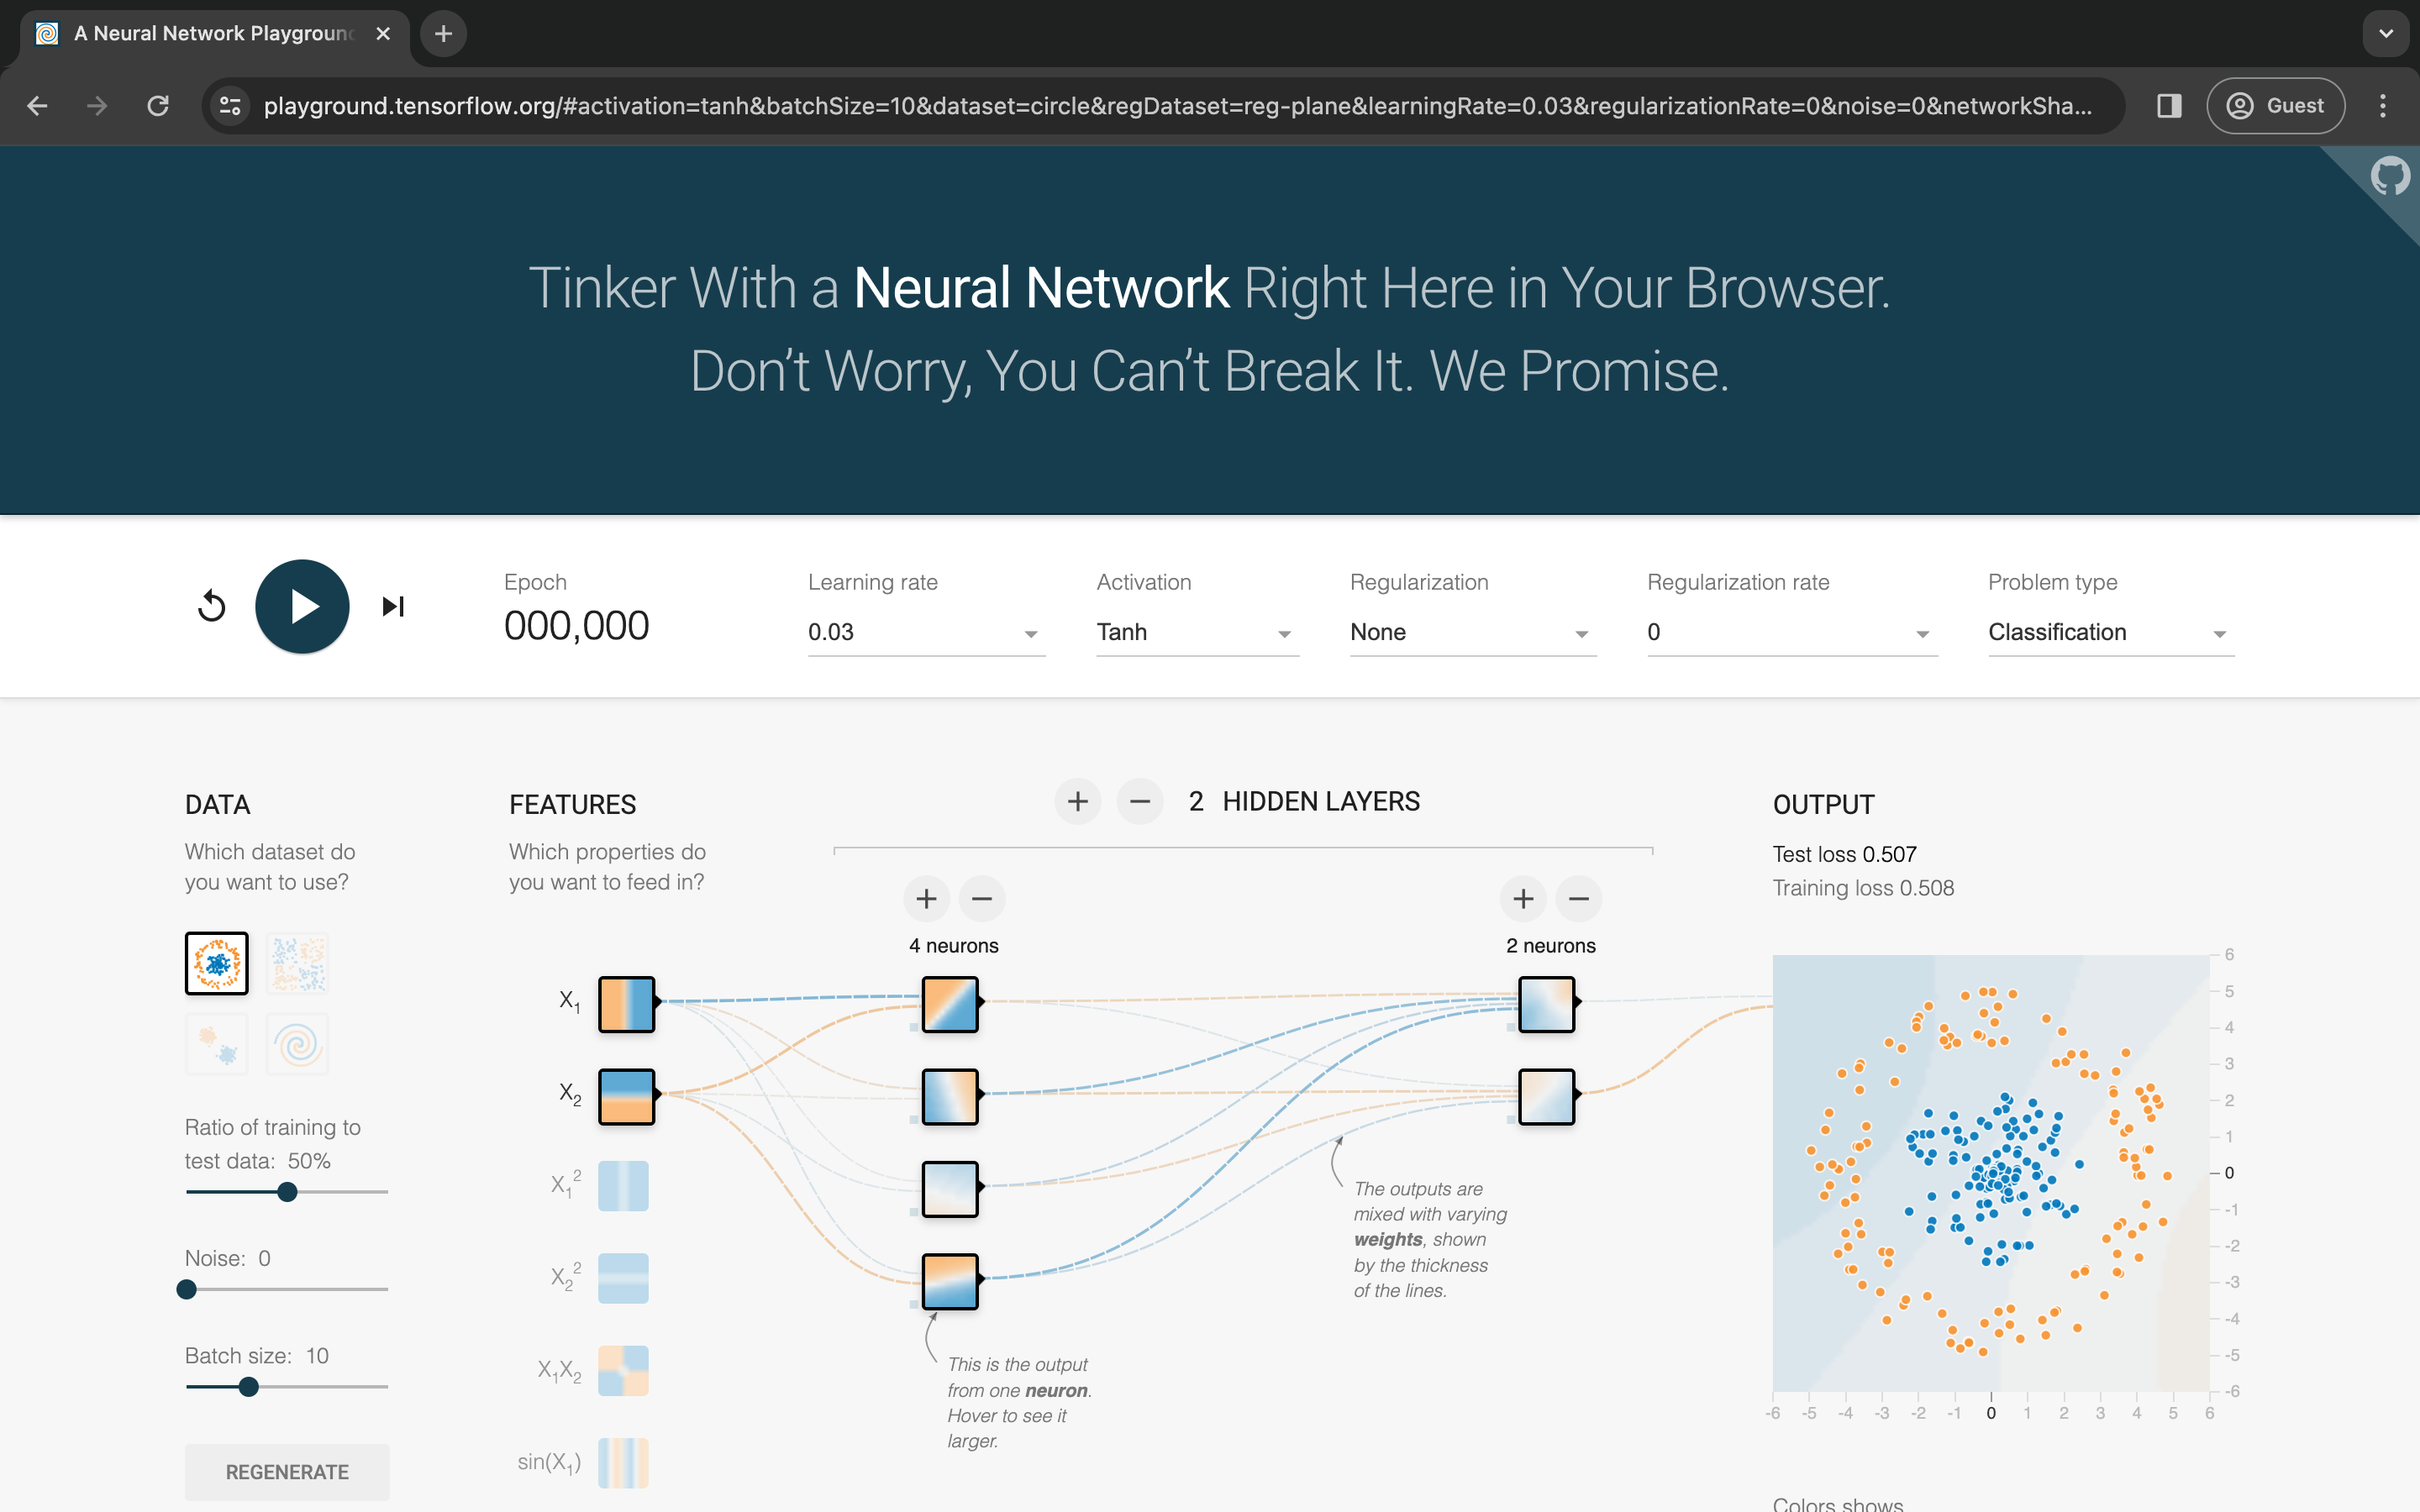
\includegraphics[width=0.4\textwidth]{./Images/tFPlayground.png}
\end{figure}
TensorFlow Playground is an free, web-browsing platform through which users are able to interact and explore nearly every aspect of neural networks. Users are able to manipulate the network's learning rate, activation, regularization, regularization rate, and problem type. It also features a written section explaining briefly what a neural network is, what aspects can be manipulated, and what is color coding means. As a browser, it definitely qualifies as a highly interactive explorable explanation. However, it requires a high level of prior knowledge to understand how to effective manipulate its plethora of controls. The explanations provided are more of an introduction to the system itself in explaining what can be manipulated but not how each manipulation will affect the output. In conclusion, its interactivity is highly engaging for those who are already educated on neural networks; however, it produces more questions than answers when shown to someone with a mere interest in the subject and on technical knowledge yet. Through a free web broser, TensorFlow Playground's accessability is decreased due to its high barrier of entry that refuses a level of opacity to those that are not trained on this topic. \cite{tensorflow2015-whitepaper}

\subsection{A Tale of 70,000 Numbers}
Jesper Fogh's thesis project at Malmo University centered around creating an explorable explanation on neural networks for users with no professional experience in computer science or mathematics. His product, A Tale of 70,000 Numbers explains how neural networks function in a narrative structure. This drag-and-drop system, has users sort hand-written number in a drag and drop system, then slowly introduces neural network functions one and a time to build up the network named Augusta1800. Its implementation of the MNIST dataset, a free, opensource dataset displays the importance of choosing the right examples to include while explaining an already complex function. It is highly engaging in not only its story-telling structure but its gradual introduction to the technicalities of how a neural network functions. As a free, web-browsing platform it is highly interactive and draws users in through its story-telling. However, due to its highly-structured narrative format, Fogh was unable to implement an actual neural network. Everything was hard-coded and merely simulated the functions and steps of a neural network. \cite{ExplorableExplanation}
\begin{figure}[h]
\caption{MNIST Dataset used by Jesper Fogh's Explorable Explanation}
\centering
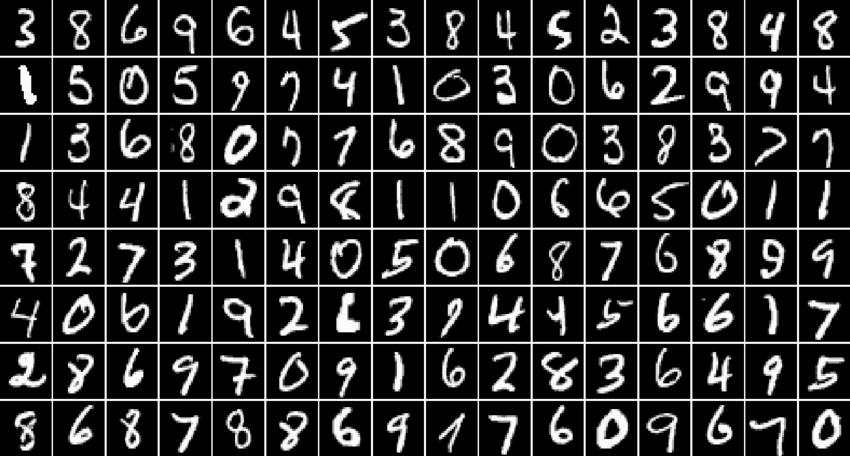
\includegraphics[width=0.4\textwidth]{./Images/mnistDataset.png}
\end{figure}

\subsection{CNN Explainer}

\begin{figure}[h]
\caption{CNN Explainer, a free, web-based Explorable Explanation centered around CNNs}
\centering
\includegraphics[width=0.4\textwidth]{./Images/CNNExplorer.png}
\end{figure}

In 2020, a group of scientists hoped to address the lack of opacity in education when learning and teaching how a CNN functions by creating a free, web-browsing platform to address challenges that non-professionals face when learning about CNNs. Their solution was to both dispally the global structure of CNNs and local layer options in an interactive and visual manner. It highly resembles TensorFlow Playground's layout: It has a highly interactive section at the top of the page followed by a description of its functions below. It improves upon TensorFlow playground by explaining key vocabulary along with pictures in its explanations. However, its separation between interaction and reading removes the explorable explanation's goal to encourage active reading. \cite{cnnExplorable}

\subsection{3Blue1Brown Videos}
Though not an explorable explanation, I included 3Blue1Brown's videos as it is one of the most prevalant educational sources when learning about convolutional neural networks. His videos include in depth explanations of vocabulary and mathematics alongside eye-catching and easy-to-understand visuals. The two alongside each other create a cohesive and comprehensive explanation of CNNs for people without and educational background in the subject. \cite{3Blue1Brown}

\subsection{Applications}
For the outcome of this project, I intend to create a convolutional neural network explanation that builds upon already-existing work in recognizing their pros and cons. From TensorFlow Playground, I hope to include a similar structure of watching a neural network function in real time, making calculations as the user interacts with it at their own pace. However, due to the confusing nature of its function without pre-existing knowledge, I intend to draw on A Tale of 70,000 Numbers's use of easy-to-consume examples in implementing the MNIST dataset, focusing my explorable explanation on processing hand-written numbers. \cite{ExplorableExplanation} In implementing the MNIST Dataset to train the CNN, I hope to model CNN Explainer's clear vocabulary definitions so that even users without a computer science or mathematical background are able to follow the explorable explanation. \cite{cnnExplorable} Lastly, I hope to implement visuals, interactivity and explanation together throughout the entire website as 3Blue1Brown does in his videos rather than separating interactivity and reading as TensorFlow Playground and CNN Explainer do. \cite{3Blue1Brown}

\section{Methods}
My design process follows a global scale and a local scale series of methods. The global scale is the step-by-step process in which the explorable explanation is actually completed. These include the following steps: define, backend coding, frontend prototyping and implementation, and user testing. The local scale for each step includes ideation, user testing, and implementation which occurs in a cyclical fashion as seen in Figure 4. This system allows for immediate reworking as opposed to finishing a product and reworking the entire project to make changes. This local system follows similarly the methodology of Fogh in his creation of A Tale of 70,000 Numbers. \cite{ExplorableExplanation}

\begin{figure}[h]
\caption{Local scale methodology of user testing}
\centering
\includegraphics[width=0.4\textwidth]{./Images/userTesting.png}
\end{figure}

\subsection{Define}
In defining my project, I follow closely to Mike Gualtieri's article, Best Practices in User Experience (UX) Design. First, I become my users. To do so, the target audience for my project needs to be specified. The result of this specification was to target users who are interested in neural networks but have no experience in the topic. Users that fit into this box were most likely junior/senior high school students and freshman/sophomore college students. With this user group in mind, I created the project with the expectation that users would come in with a basic knowledge of matrices and pre-calculus. Then, following Gualtieri's writing, I "design first to avoid leaving user experience to chance." This included creating a low-fidelity prototype or outline of my web-browser in order to specify how and what I intend to explain about CNNs as they can be and are very complex. This low-fidelity prototype was then subject to user testing in receiving feedback on if the flow of contents flow easily or not. Since a low-fidelity prototype is the mere skeleton and does not go into detail, my user testing pool consisted of students who were already knowledgeable on CNNs, having only recently learned it. This held great insight into what worked and what didn't in terms of what they appreciated and did not in their own learning experience. \cite{UXDesignHandbook}

\subsection{Backend Implementation}
The next step was ensuring that a CNN was available to use for the web-browser as it would provide most of the interactivity. This process was not only of importance to the web-browser but was instrumental in part of the background research for creating this project. Having to build a CNN forced me as the creator to analyze how much I knew about CNNs and what I had questions on so I could better create an explorable explanation for those who had no background knowledge. The methodology of this step was primarily implementing TesorFlow.js, an open source machine learning platform for Javascript and web development. Backend coding also included collecting data so that not only could the CNN be trained but so that a dataset example could be provided on the explorable explanation. Fortunately, the MNIST dataset of handwritten numbers is open source and readily available for users to access. \cite{tensorflow2015-whitepaper}

\subsection{Frontend Prototyping and Implementing}
As defined by designers Houde and Hill, a prototype is "any representation of a design idea, regardless of medium." This includes the look and feel of the product, the look and feel of each asset, and the role or function of the product. \cite{prototyping} My frontend prototyping was created through Figma (the medium), a popular interactive design tool amongst UX/UI designers. Figma allowed for the creation of a high-fidelity prototype as opposed to the low-fidelity prototype made during the ideation phase. Whereas the low-fidelity prototype contained the skeleton of the webapp, this high-fidelity prototype were the meat and skin of the product, including the text and interactive buttons so user testing could simulate the use of the real product. The user tests of the prototype included both users who had prior knowledge of CNNs and users who had no knowledge of CNNs. Their feedback ensured that the interactive elements which were not present in the low-fidelity prototype made logical sense and that the layout of the site transitioned smoothly from one section to another, ensuring each asset had role and an intuition look/feel to it. 


The final implementation process of a free web-browser was done through HTML, javascript, and CSS. Prototyping the website beforehand was essential to the implementation of the website as in ensured at all design choices were solidified beforehand and no design work would be necessary whilst coding. The web browser was coded locally, meaning it was only accessible through my laptop. Once the web browser was completed locally, it then uploaded onto Render, a free, unified cloud to build and run web applications. This allowed for the website to be accessible to anyone with access to the link, making it a fully functioning explorable explanation. 

\subsection{User Testing}
The process of user testing was done through a survey sent out to various potential users. A link to the website and survey was sent out to 50 potential users. The results from the survey were then collected onto an excel sheet to find the average response. 

\section{Evaluation Metrics}
My project consisted of two key compartments that required evaluation metrics: the backend and the frontend. The backend evaluation consisted of ensuring that my CNN implemented to the website was consistent and accurate. The frontend evaluation consisten of following my user testing methodology of surverys in order to receive data on how impactful and accessible the explorable explanation is. Both work in tandem to increase opacity toward black box models in revealing the accurate functions of a convolutional neural network. 

\subsection{Backend Evaluation Metrics}
In implementing a CNN as the backend of the explorable explanation, I employed the use of TensorFlow. To evaluate my CNN built by reading TensorFlow documentation and implementing its libraries, I am implementing a comparative evaluation metric between three different neural networks built for image categorization for the MNIST dataset.


First off, I created a separate neural network from scratch on Python following a tutorial by Samson Zhang. \cite{pythonCNNScratch} I then created a CNN on Python with TensorFlow. And lastly, created the Javascript CNN with Tensorflow.js. All three neural networks were trained on the same MNIST dataset. I ran each neural network several times, comparing their accuracy. This formulated the evaluation method of the backend. I considered the neural networks to be accurate if the margin of error fell between 4 to 8 percent with a 95 percent confidence level. \cite{tensorflow2015-whitepaper}

\subsection{Frontend Evaluation Metrics}
As a project designing and creating an explorable explanation, most of the evaluation work occurs for the front-end. Due to the subject nature of UX design metrics, my evaluation mostly consisted of survey results with a mix of both quantitative and qualitative results. These results were then taken and averaged both in terms of numbers and sentiments in order to produce results for the project. 

\begin{figure}[h]
\caption{Four Categories of Analysis for Explorable Explanations}
\centering
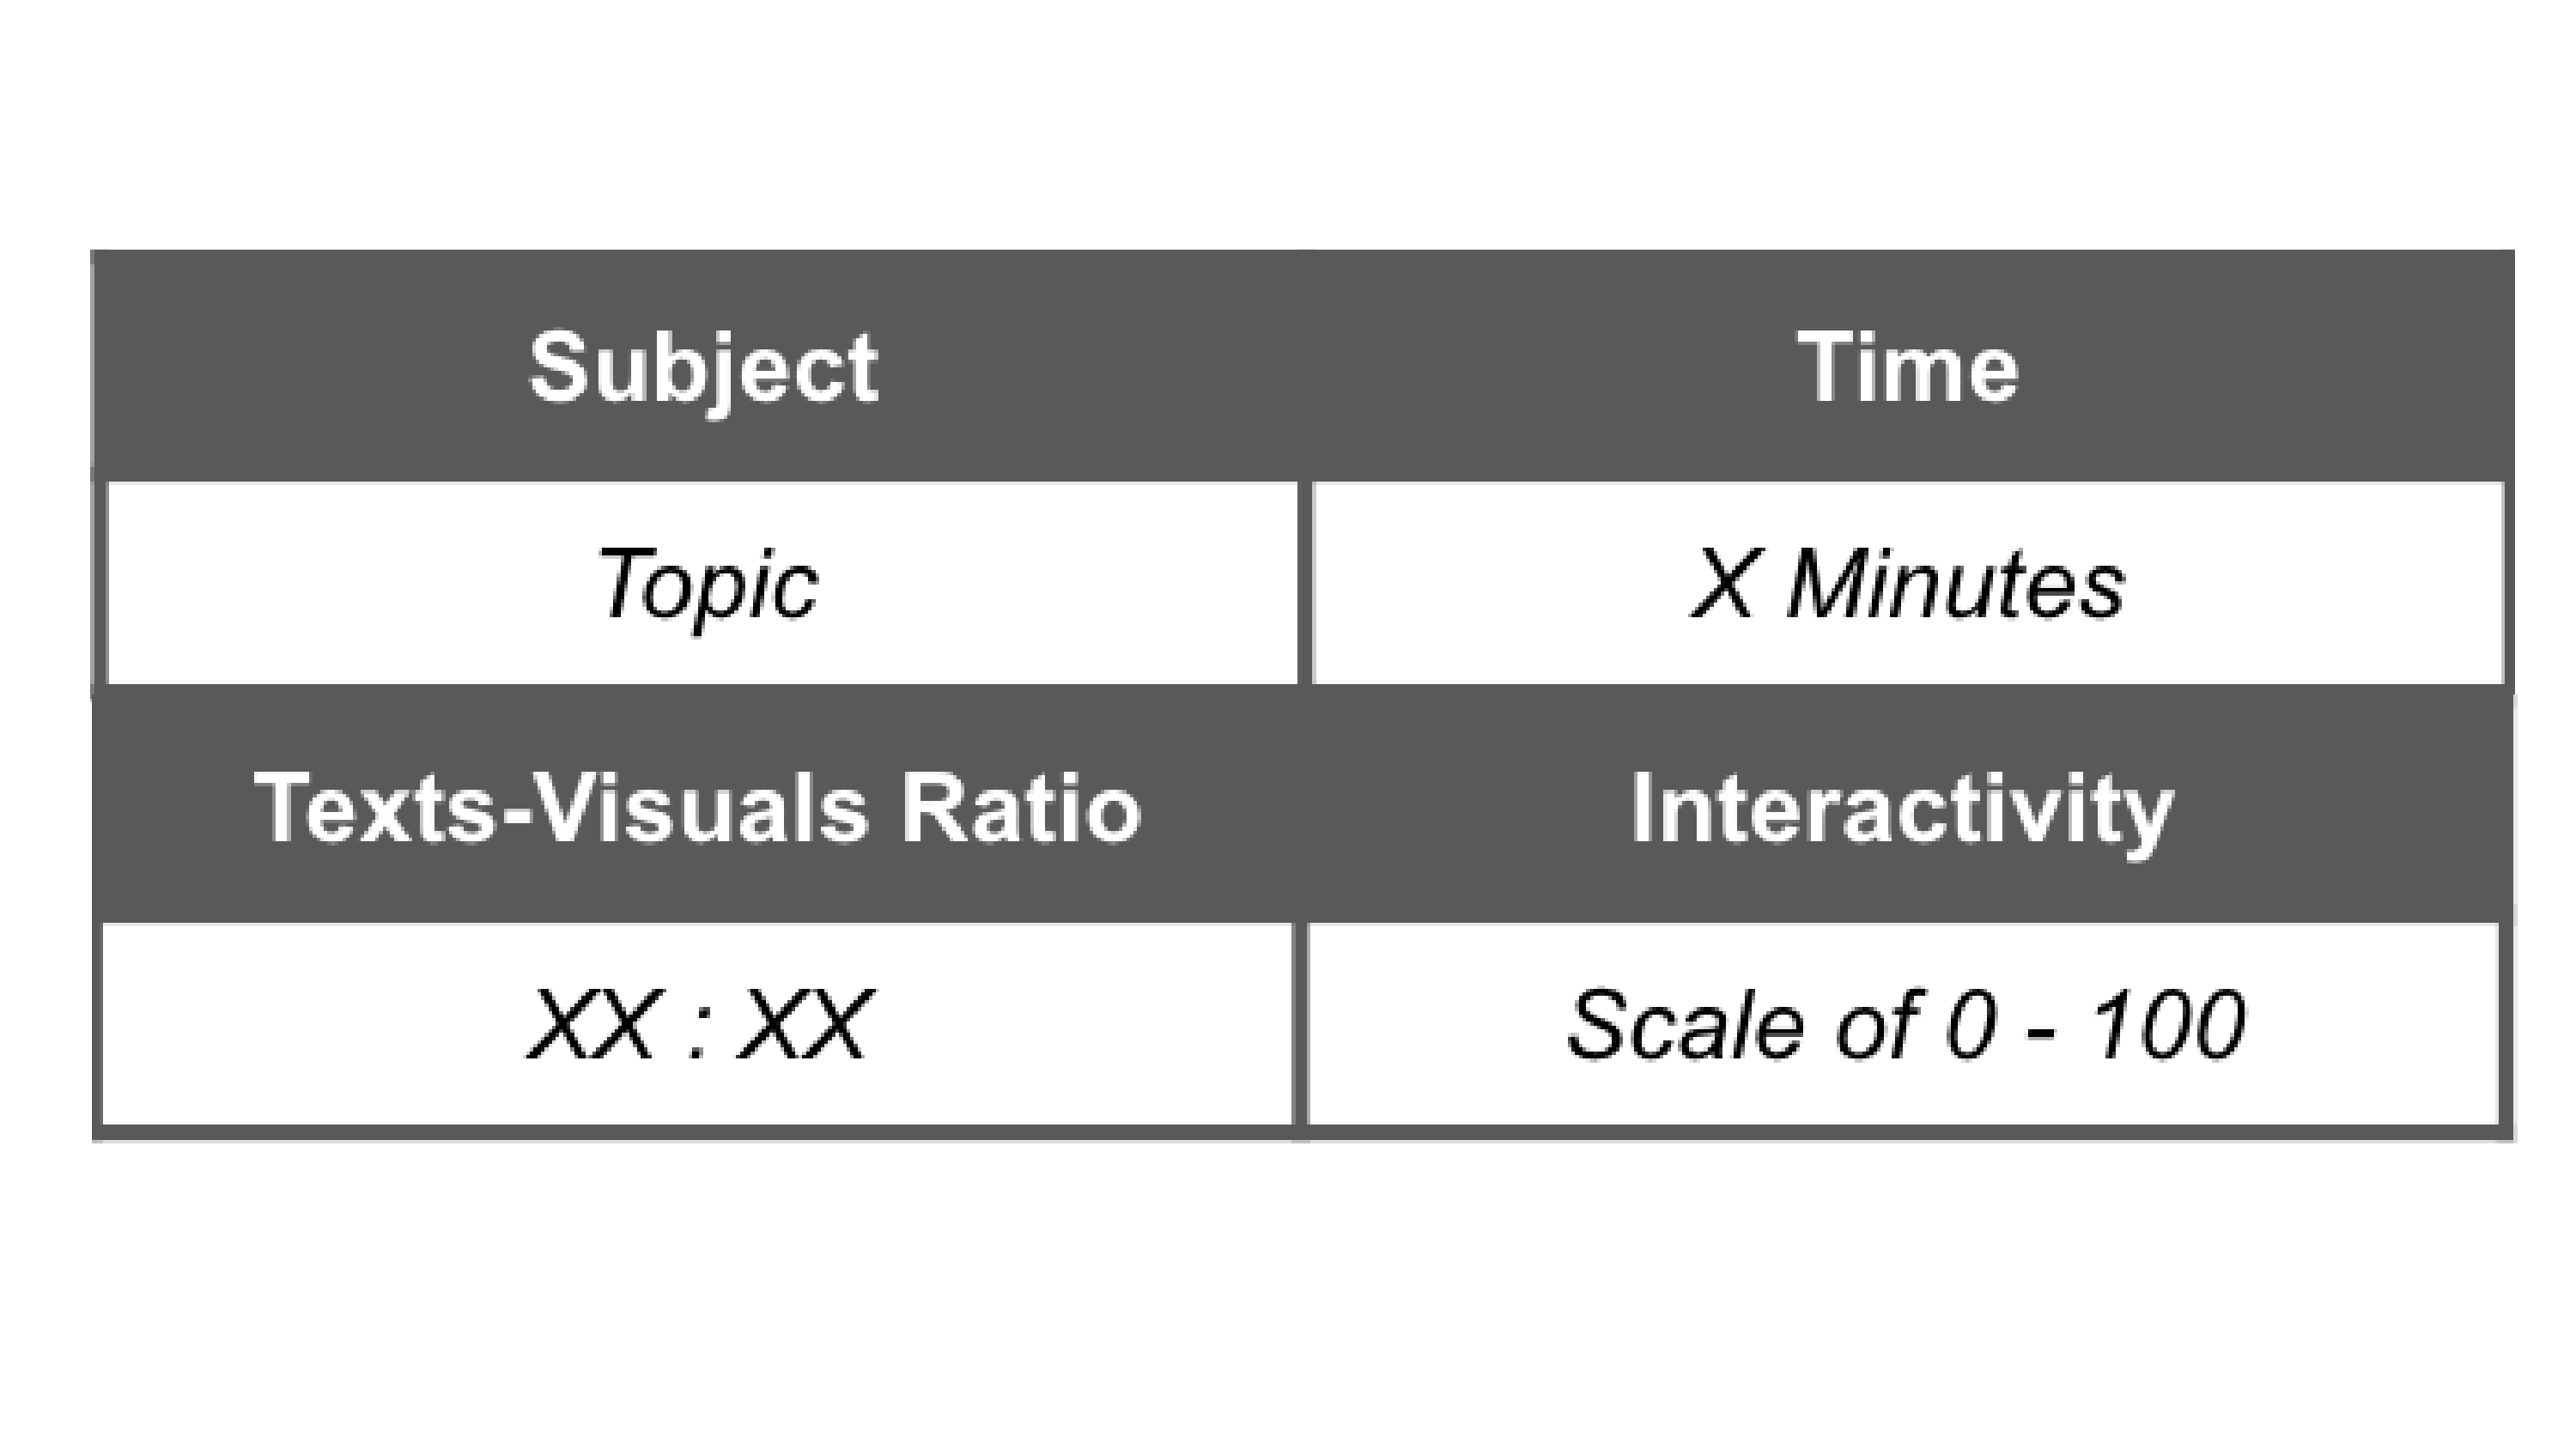
\includegraphics[width=0.4\textwidth]{./Images/categoriesOfAnalysis.pdf}
\end{figure}

In terms of quantitative results, I looked at the four categories of analysis for explorable explanations: topic, time taken, text-to-visual ratio, and interactivity (visit Figure 5). For topic, users were asked to succinctly write down what the topic of the explorable explanation was--what was it trying to explain? For time taken, users were asked to record how long the explorable explanation took for them to follow. The ideal time for the explorable explanation was ten minutes as the explorable explanation aimed for accessability which includes easily consumable content that people could look over fairly fast and learn from. This goal also aims to decrease the entry of barrier to machine learning as a long document could be intimidating and drive away viewers. Text-to-visual ratio represents the ratio between reading elements and interactive elements or images. The average ratio between text-to-visuals in explorable explanations is 46:54. As such I aimed for my text-to-visual ratio to average around 50:50 balancing both equally as I knew that a lot of my text would center around explaining vocabulary and background knowledge as a cite for beginners without prior knowledge. Lastly, amount of interaction (interactivity) is rated on a scale of zero to 100. Interactivity reflects how much the user is able to affects the contents on screen, for example highlighting text or displaying images. \cite{ExplorableExplanation}


In terms of qualitative results, the survey also includes several short answer questions that allow for users to voice their subjective experience using the explorable explanation. Such questions focus more on highest cognitive dimension along with user satisfaction. Cognitive dimension ranges is comprised of six parts: remembering, understanding, applying, analyzing, evaluating, and creating. My project hopes to reach the second cognitive dimension of remembering and understanding as I aim for this project to provide users a basic introduction to CNNs. Higher cognitive dimensions require higher levels of understanding and explanation that the explorable explanation ideally inspires users to explore and makes it feel reachable. \cite{cognitiveDimension} In terms of user satisfaction, it looks at intuitive the explorable explanation was to move through. The goal is to avoid confusion in not only the explanation of how CNNs work but also in the physical navigation of the cite. The two, cognitive dimension and user satisfaction function in a feedback loop, as a higher cognitive dimension reached for users reflects a higher user satisfaction and high satisfaction in web navigation allows for users to reach a higher cognitive dimension of understanding what CNNs are. \cite{ExplorableExplanation} Together, a positive qualitative response reflects an increase in opacity towards CNNs as it bridges the original "mismatch between mathematical optimization and high-dimensionality characteristics of machine learning and the demands of human-scale reason and styles of semantic interpretation." 
\cite{MLOpacity} 

\section{Results and Discussion}
The project was completed to its fullest within the time frame of 15 weeks. As it currently stands it qualifies as an explorable explanation per the definition stated previously in our technical background. The finalized website is title 'Dear Neural Networks, What the F*ck Are You' as an attempt to connect with users in a more candid manner as opposed to the commonly seen, highly technical titles of papers and articles on machine learning. The following sections will delve into results from both backend and frontend evaluations, followed by a discussion on how user feedback can be implemented moving forward to improve the explorable explanation in terms of both accessibility and opacity. 

\begin{figure}[h]
\caption{Title Page of Final Product}
\centering

\includegraphics[width=0.4\textwidth]{./Images/titlePage.png}
\end{figure}

\subsection{Backend Results}
Three function neural networks were created as a part of the comparative evaluation to ensure the accuracy of our backend: one neural network coded from scratch on Python, one coded with TensorFlow on python, and one coded with TensorFlow on Javascript. I ran each code ten time, took the average accuracy of all three. The margin of error between the three neural networks's accuracy was found to be five percent error with a 95 percent confidence. This fulfills the original evaluation method of the margin of error falling between four to eight percent error with a 95 percent margin of error. 

\subsection{Backend Discussion}
In analyzing the results of the backend evaluations, I realize that it would be ideal for there to exist a python code made from scratch for a CNN as opposed to a two-layered neural network. Since a two-layer neural network lacks much of the complexity of a CNN, namely the convolution layer, the accuracy of it was much lower than either of the CNNs made with TensorFlow. However, the complexities of building a CNN completely from scratch with numpy and math would have qualified as its own project over the course of 15 weeks. However, this process of cross-comparison between the three neural networks was extremely useful in dissection the difference between CNNs as opposed to other networks in deep learning. 

\subsection{Frontend Results}
Though implementing one's own neural network code is the ideal way to understand it, the job of the frontend was to relay this experience, providing that opacity without users having to go through the tribulations and intimidation of building one's own CNN. However, an analysis of the frontend evaluations are required. Not all 50 users responded to the survey, resulting only in a pool of 30 submitted surveys. 
\begin{figure}[h]
\caption{Explorable Explanation accessed online, published through Render}
\centering
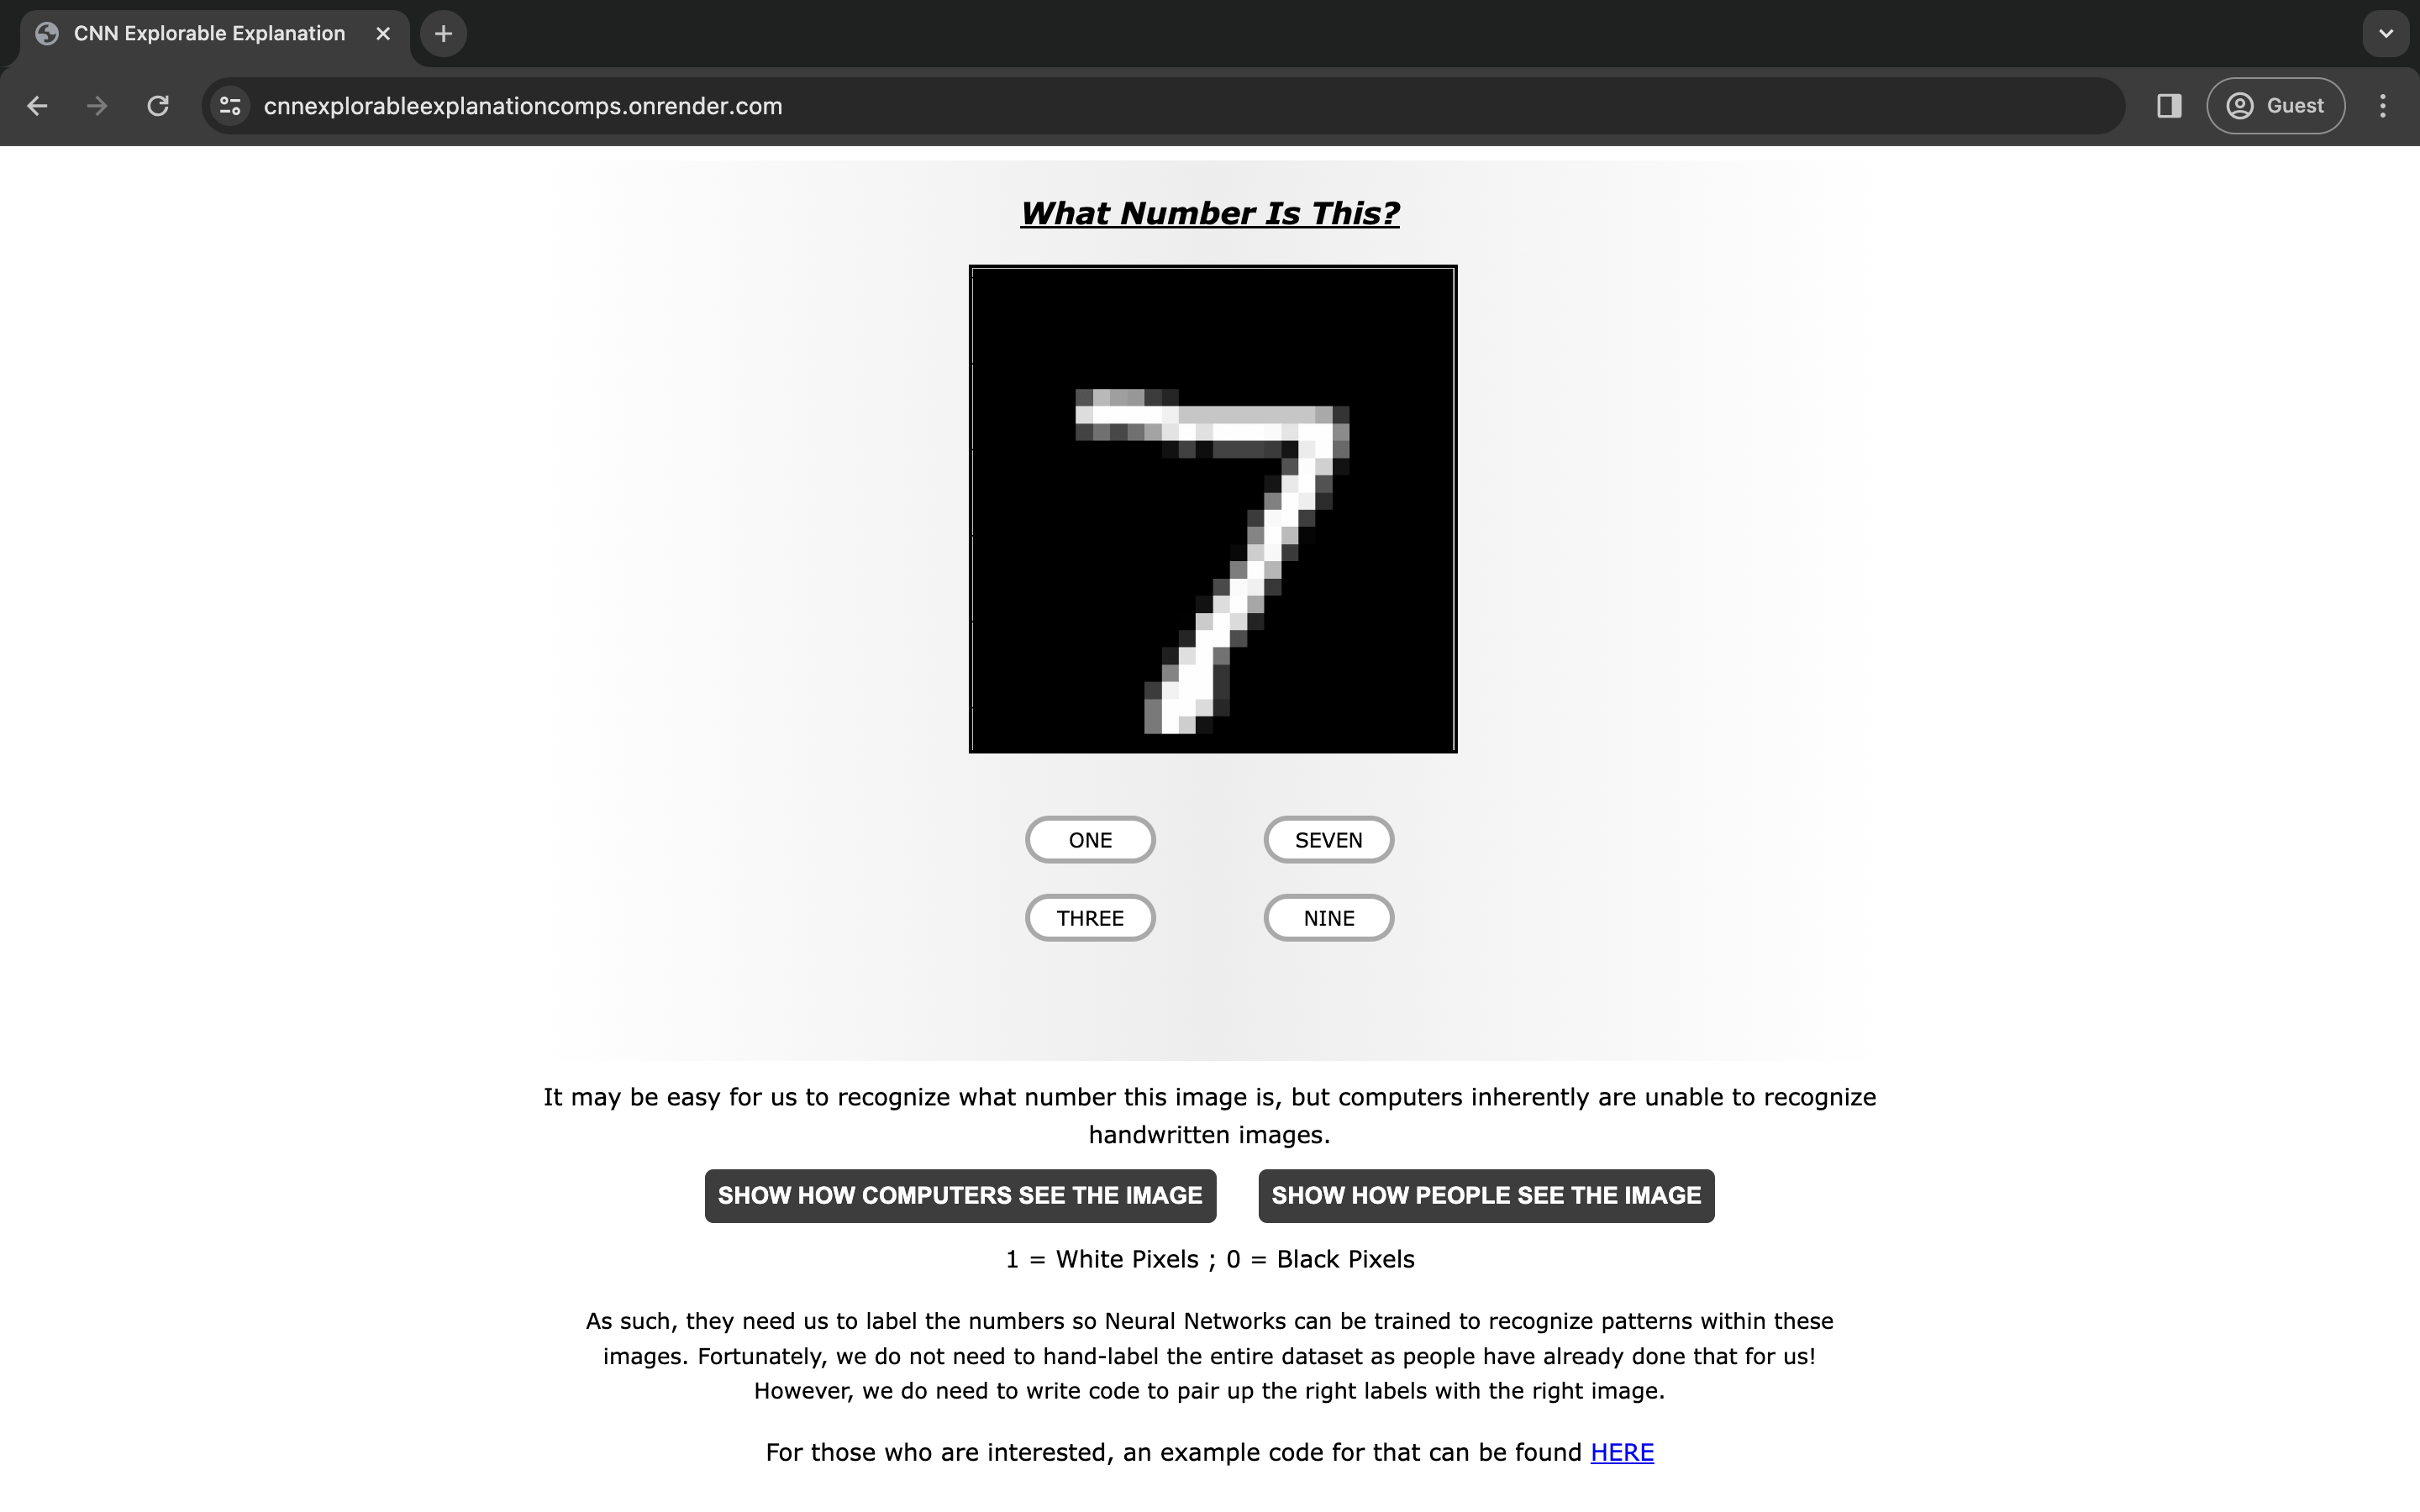
\includegraphics[width=0.4\textwidth]{./Images/ExampleScreenShot.png}
\end{figure}
\subsubsection{Quantitative Results}
The average amount of time spent on the explorable explanation averaged around 9.28 minutes, which achieved my goal of under ten minutes. The average text-to-visual was found to be 55:45. Unfortunately, the ratio leaned more towards text than visual as I inteded a 50:50 ratio. Lastly, the interactivity had an average rating of 82 percent. 
\subsubsection{Qualitative Results}
Questions that asked users what they learned and how much they learned about convolutional neural network relayed a fairly high level of cognitive dimensionality in respect to my desired level of understanding. Of the 30 users, 23 users were able to accurately label the topic of the explorable explanation as 'convolutional neural network'; however, seven users reported the topic as 'neural network'. Though the response is correct, I really wished to clarify the fact that a convolutional neural network is only one type of network in the wide varieties of networks that exist in deep learning. They reflected a new understanding of how layers worked in neural networks and a newfound understanding of how computers process images through a numerical system. 


In terms of user satisfaction. There was a positive response to the flow of the website from explaining vocabulary first then moving onward to a real-time example. Based on feedbaack, each interactive element was intutitive and easy to work with. There was mixed feedback on the general look of the website. Some responded, stating that they liked the minimalistic black and white layout of the website as it highlighted visuals. However, others responded with a  desire for more color in the design to increase engagement and interest from the user's perspective.

\begin{figure}[h]
\caption{Example of CNN Running in Real Time from 'Dear Neural Networks, What the F*ck Are You}
\centering
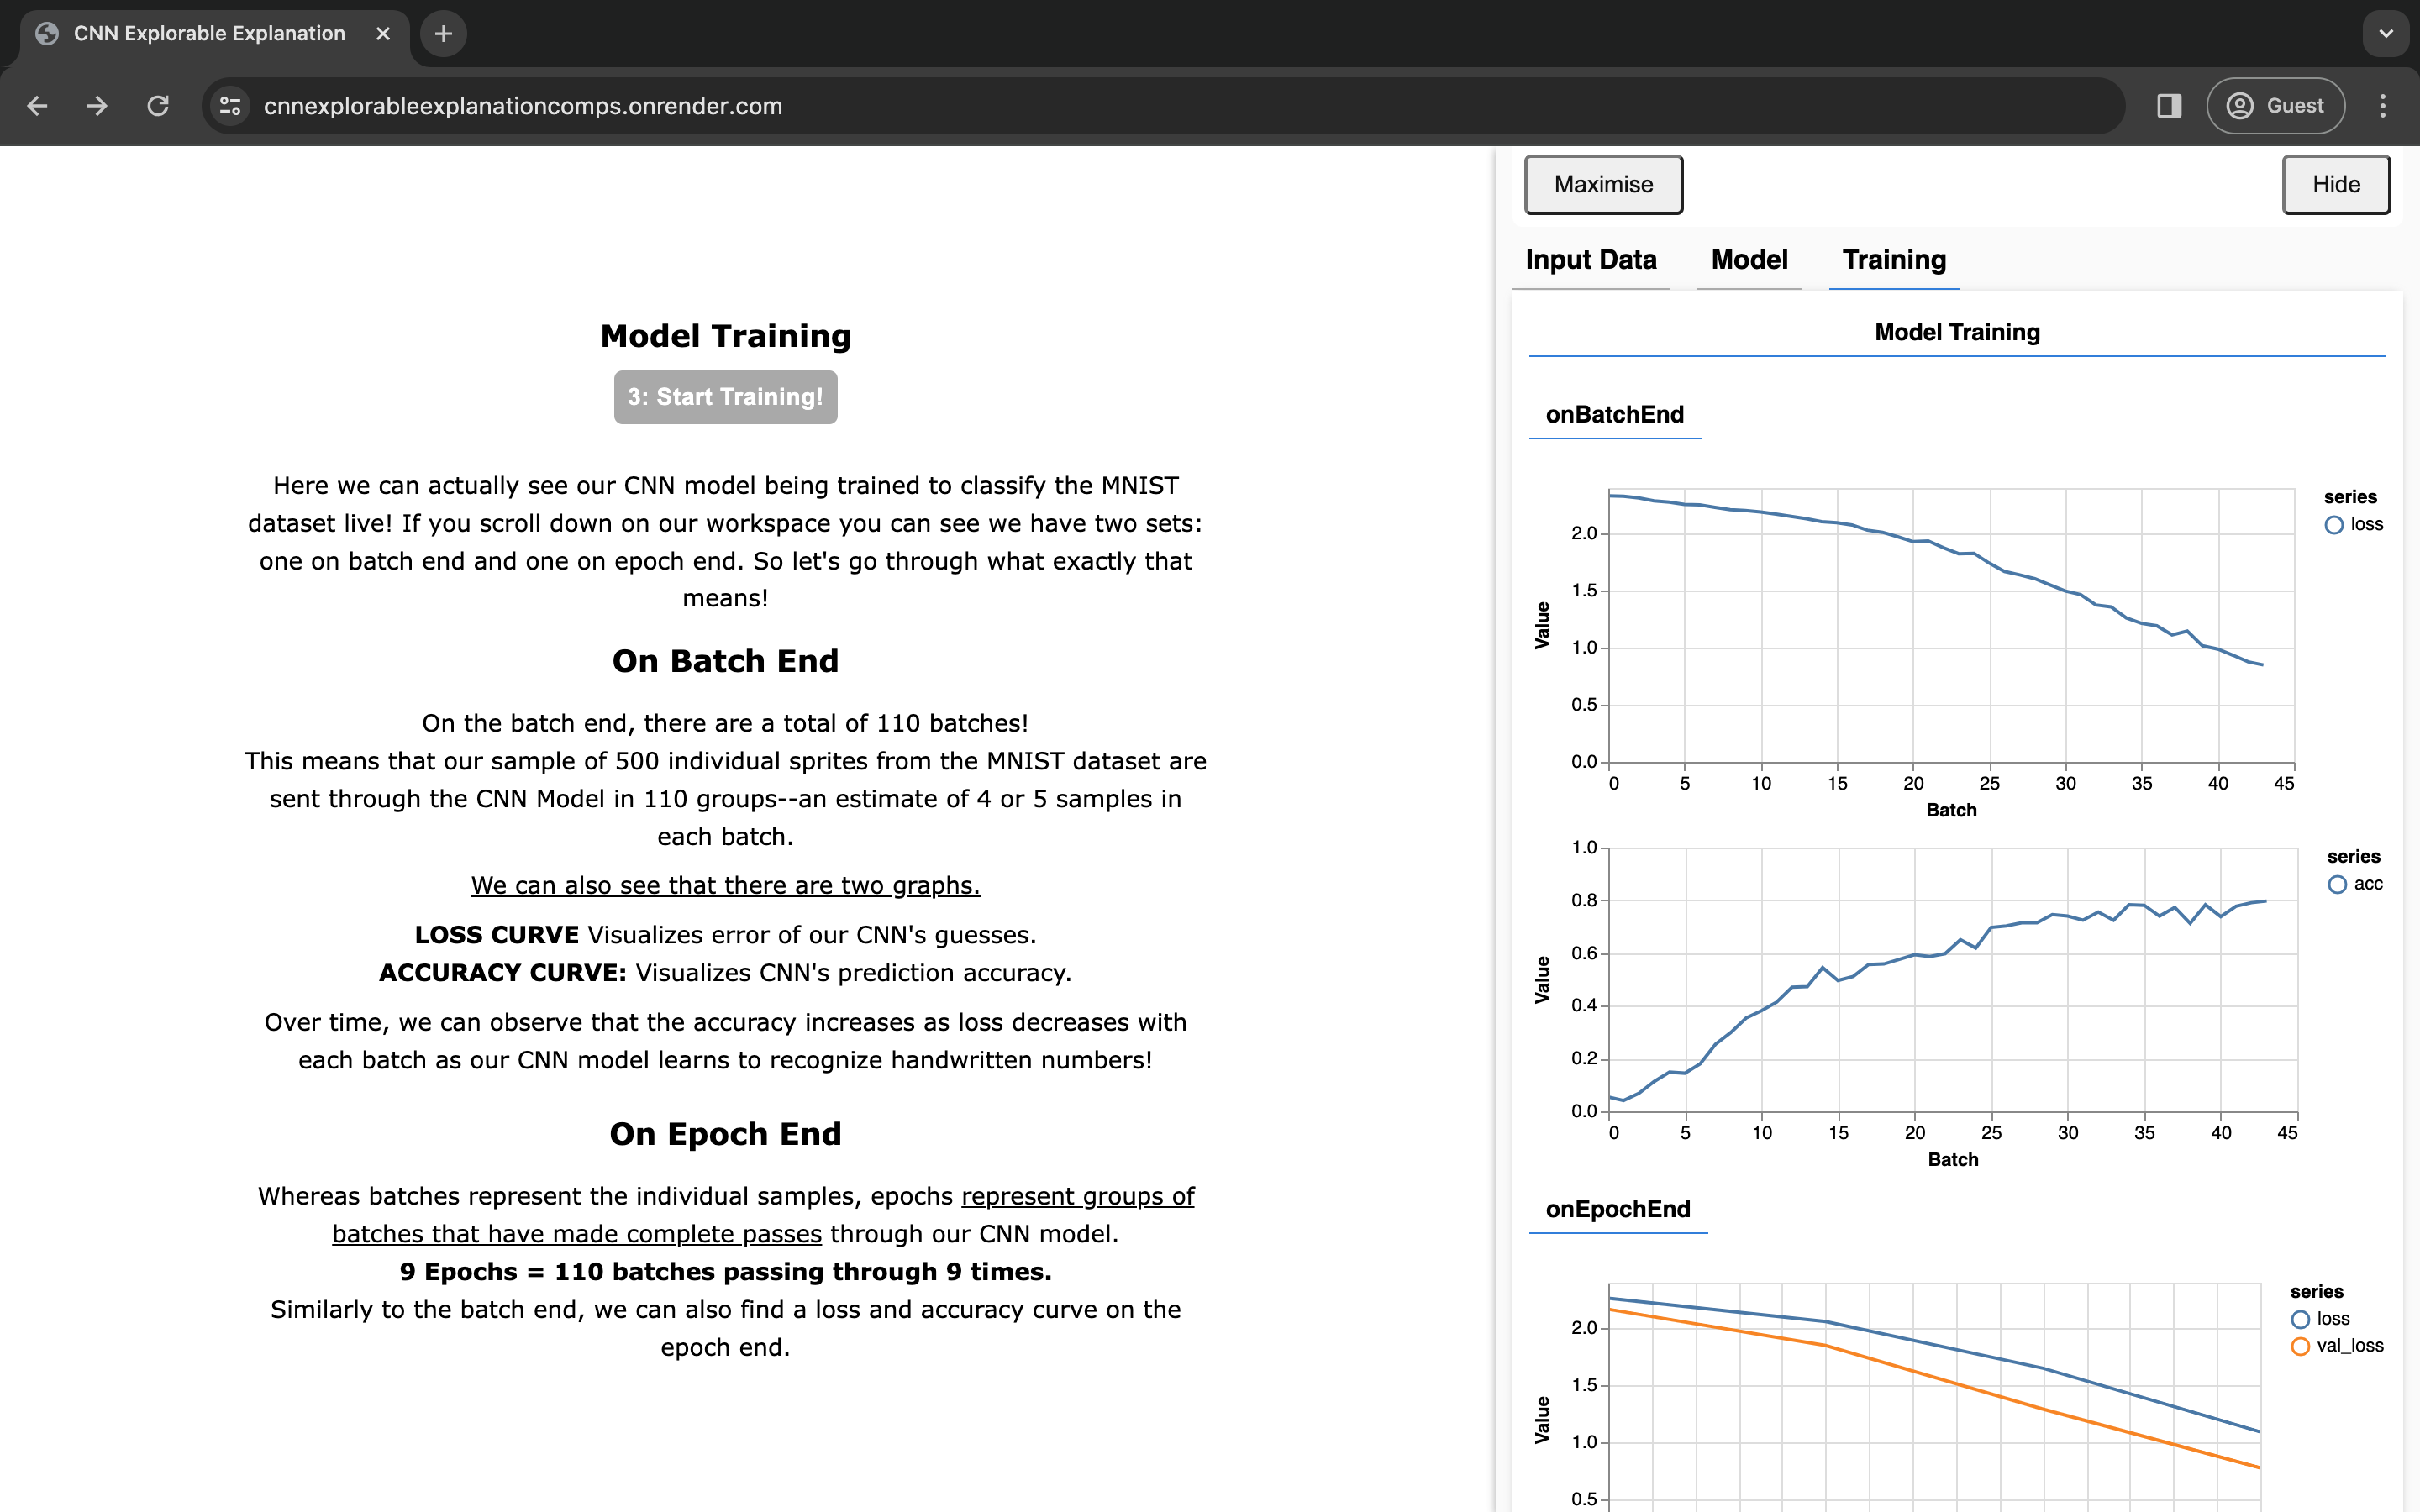
\includegraphics[width=0.4\textwidth]{./Images/realTimeCNN.png}
\end{figure}

\subsection{Frontend Discussion}
Overall, there was a positive response to the explorable explanation 'Dear Neural Networks, What the F*ck Are You?'. It hit nearly all my quantitative and qulitative goals aside from the text-to-visual ratio. As a way to increase interactivity to the website, added interactive elements beyond buttons would be ideal. By having different forms of interactivity, it can engage users further as it keeps users looking forward to what the next interaction is. I originally inteded to have a section where users could input their own sample data, writing a number and submitting it. However, due to time constraints, I was unable to complete this function for the website. Despite the positive feedback from the sample of surveys I received, there are multiple changes that could have been made to the user testing process that ensures a less biased set of results. This will be further discussed in the following ethical considerations. 
\begin{figure}[h]
\caption{Example of text to visual comparison from 'Dear Neural Networks, What the F*ck Are You'}
\centering
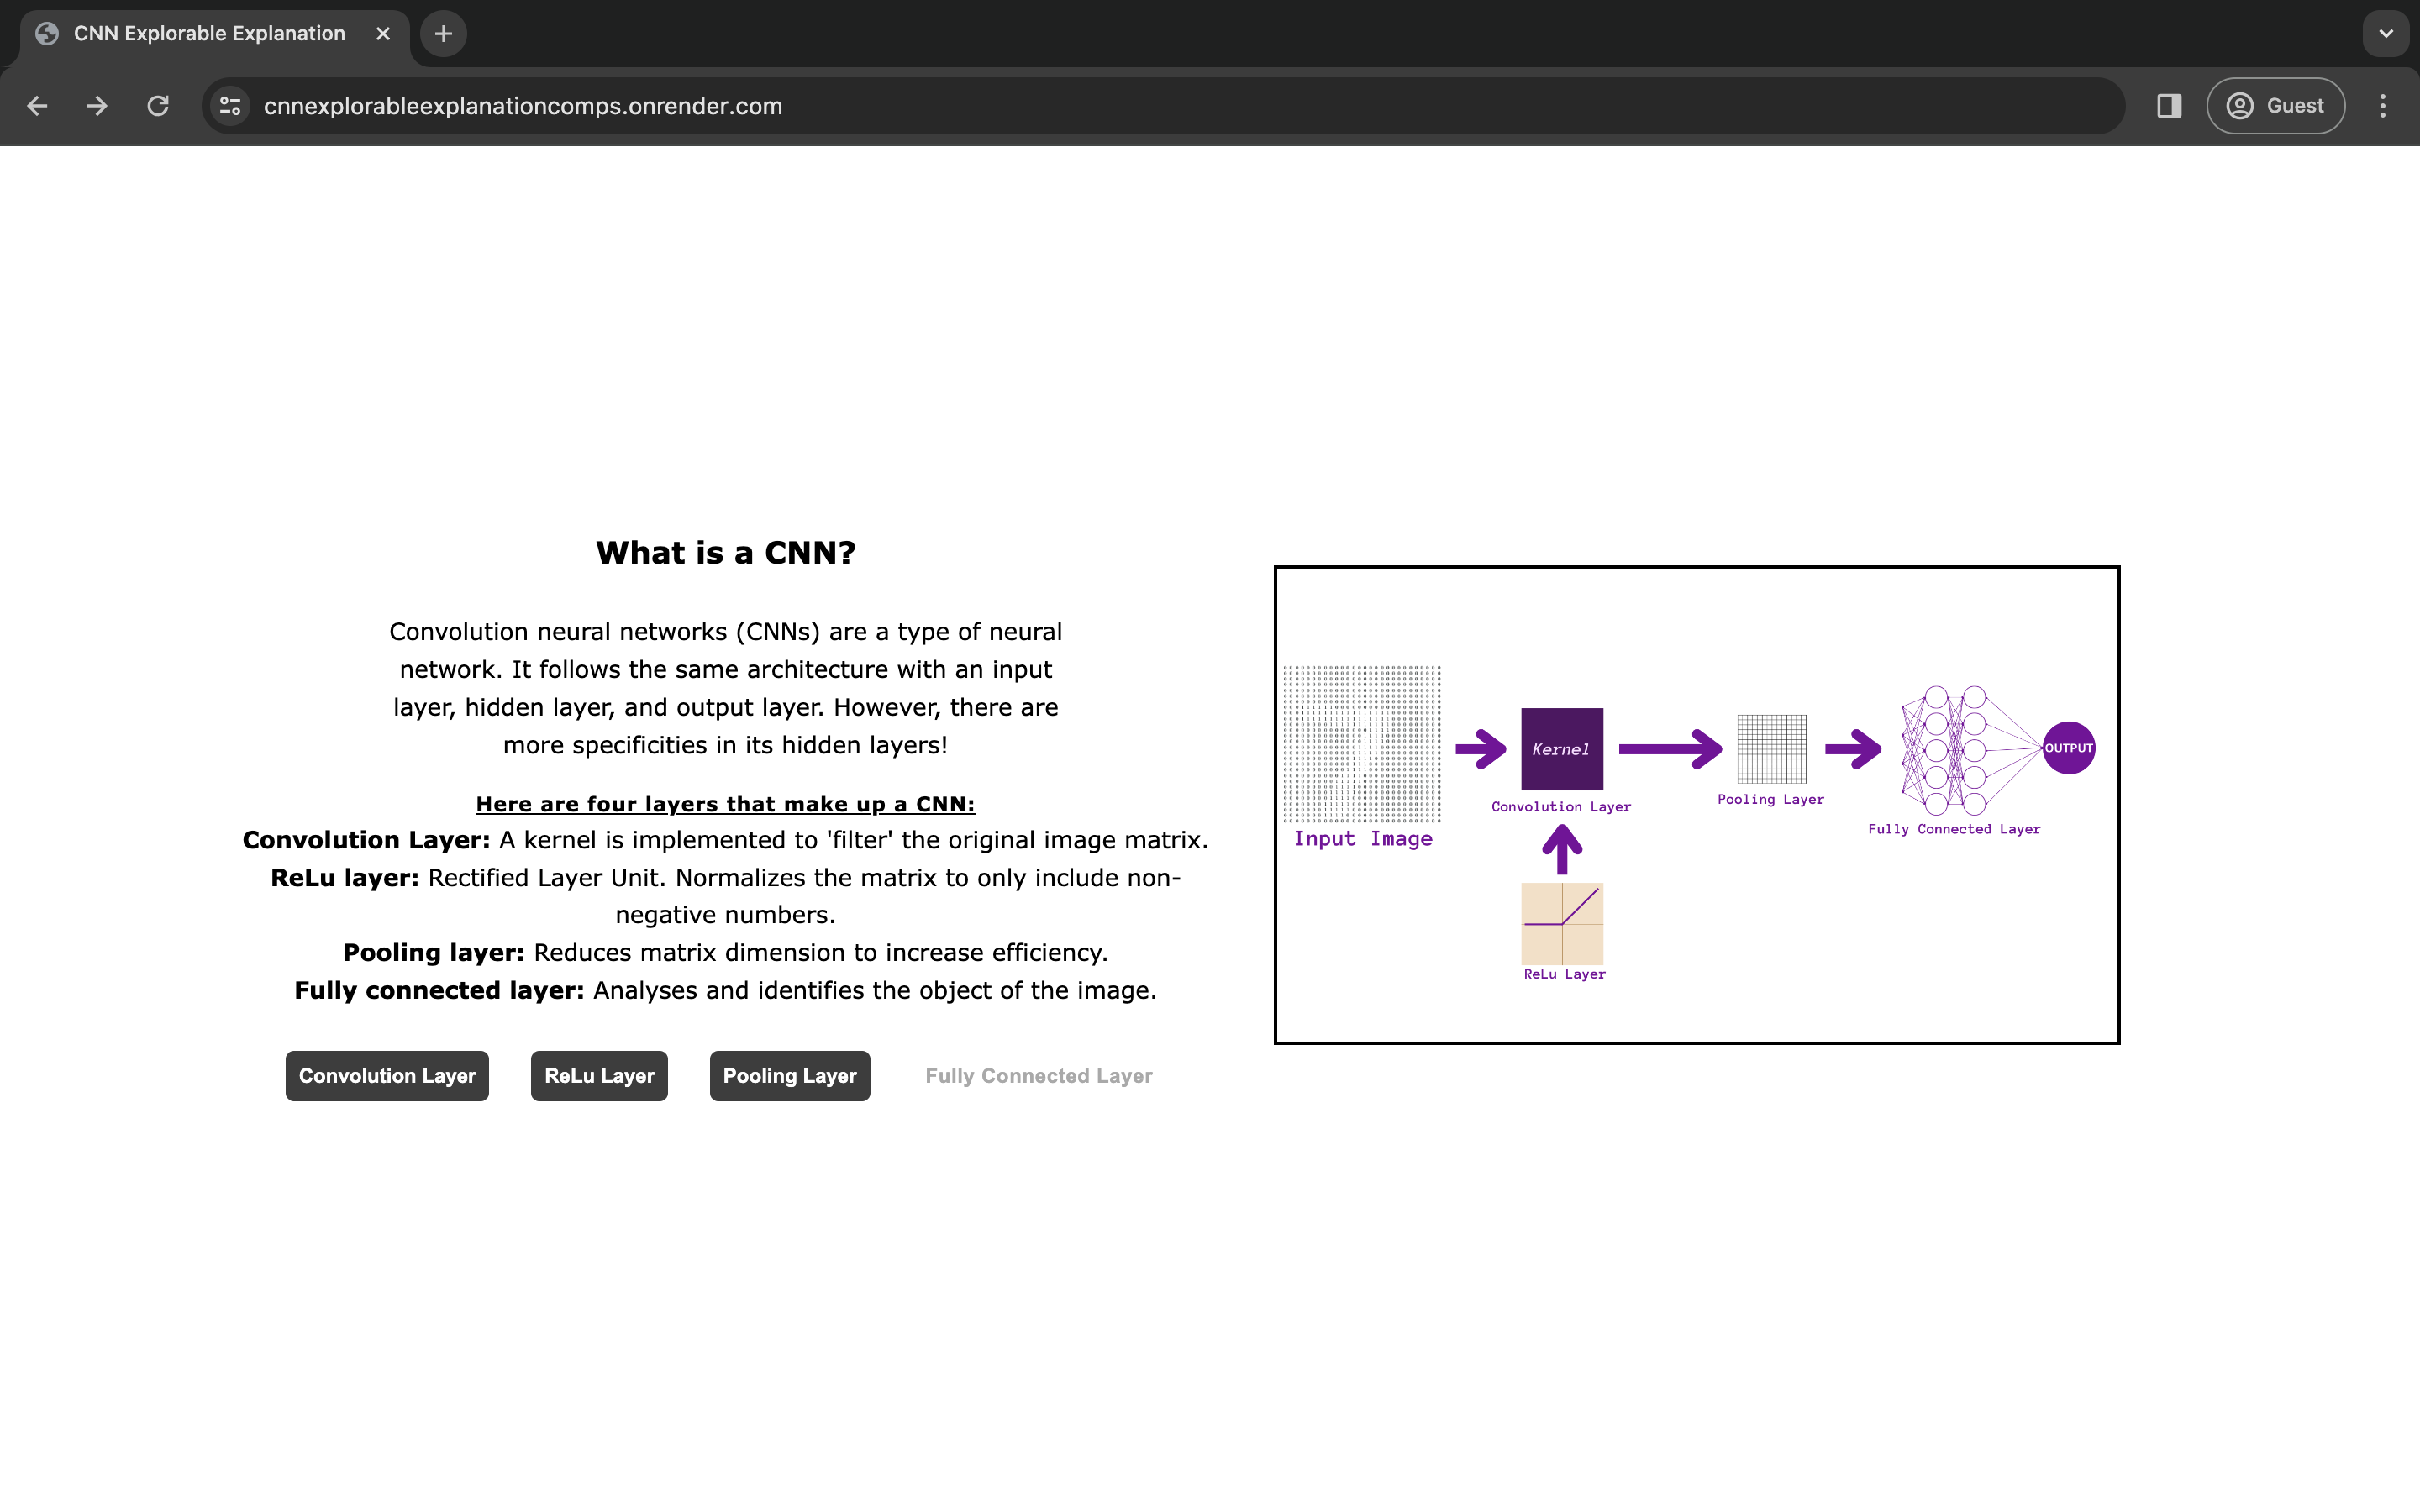
\includegraphics[width=0.4\textwidth]{./Images/textToVisual.png}
\end{figure}

\section{Ethical Considerations}
As a UX/UI design project that centers most of its evaluations around user testing, there are several ethical considerations with the surveying process implemented for this project. Beyond user testing, there are also certain considerations to be made in the actual content on the website and design aspects implemented. 
\subsection{User Testing Considerations}
In Fogh's user research process for A Tale of 70,000 Numbers, he implemented in-person testing and interviews on his explorable explanation. \cite{ExplorableExplanation} However, due to timing, my user-testing process took place over Thanksgiving break in which most potential users were not in my vicinity. This resulted in a need for surveys and as such, limited responses on my user testing result. By having in-person tests and interviews I would have been able to receive a fuller scope on how users interacted with the website and what troubles they might have encountered. Fogh's request for users to voice their thoughts and opinions as they tested the website would have been of value in this aspect. 


My questioning in the survey also could have been more specific as opposed to open-ended questions like "what did you learn from this explorable explanation." By asking such open ended questions, I am unable to understand the full scope and impact or lack thereof of the explorable explanation. Since I was unable to hold in-person testing and interviews, I also should have made a better effort to send the survey and website to people outside of my local OXY community. This very much limited the pool of people and did not provide an accurate representation of the general public who have a very different relationship-or lack thereof-with technology since students at Occidental College to come with a certain level of privilege in their access to and in turn knowledge of technology.

\subsection{UX Design Considerations}
One of the largest criticisms I received in my presentation of the project was about the font size. This was especially prevalent for professors that looked at the project. Due to the fact that my identified primary users were high school and college students, I did not account for the possibility of age in my UX design process. For those of generations beyond the high school to college age range, it is important to account for eyesight as a form of accessibility. This is true even for people of the younger generation who may be born with certain visual difficulties. It was not until after the project was finalized that I reached this realization and found Accessibility for Teams, a framework published by the US government on proper UX design standards for accessibility. Under U.S. Web Design Standards (USWDS) Typography, it states, "For most texts, including body copy, use at least an effective size 16px." \cite{typography} As it currently stands, the website body text is 12px, far under the expected 16px (visit Figure 10). As a part of ethical design, I should have sought out USWDS standards earlier in my process of prototyping. 
\begin{figure}[h]
\caption{Font in 12px as opposed to the effective size 16px}
\centering
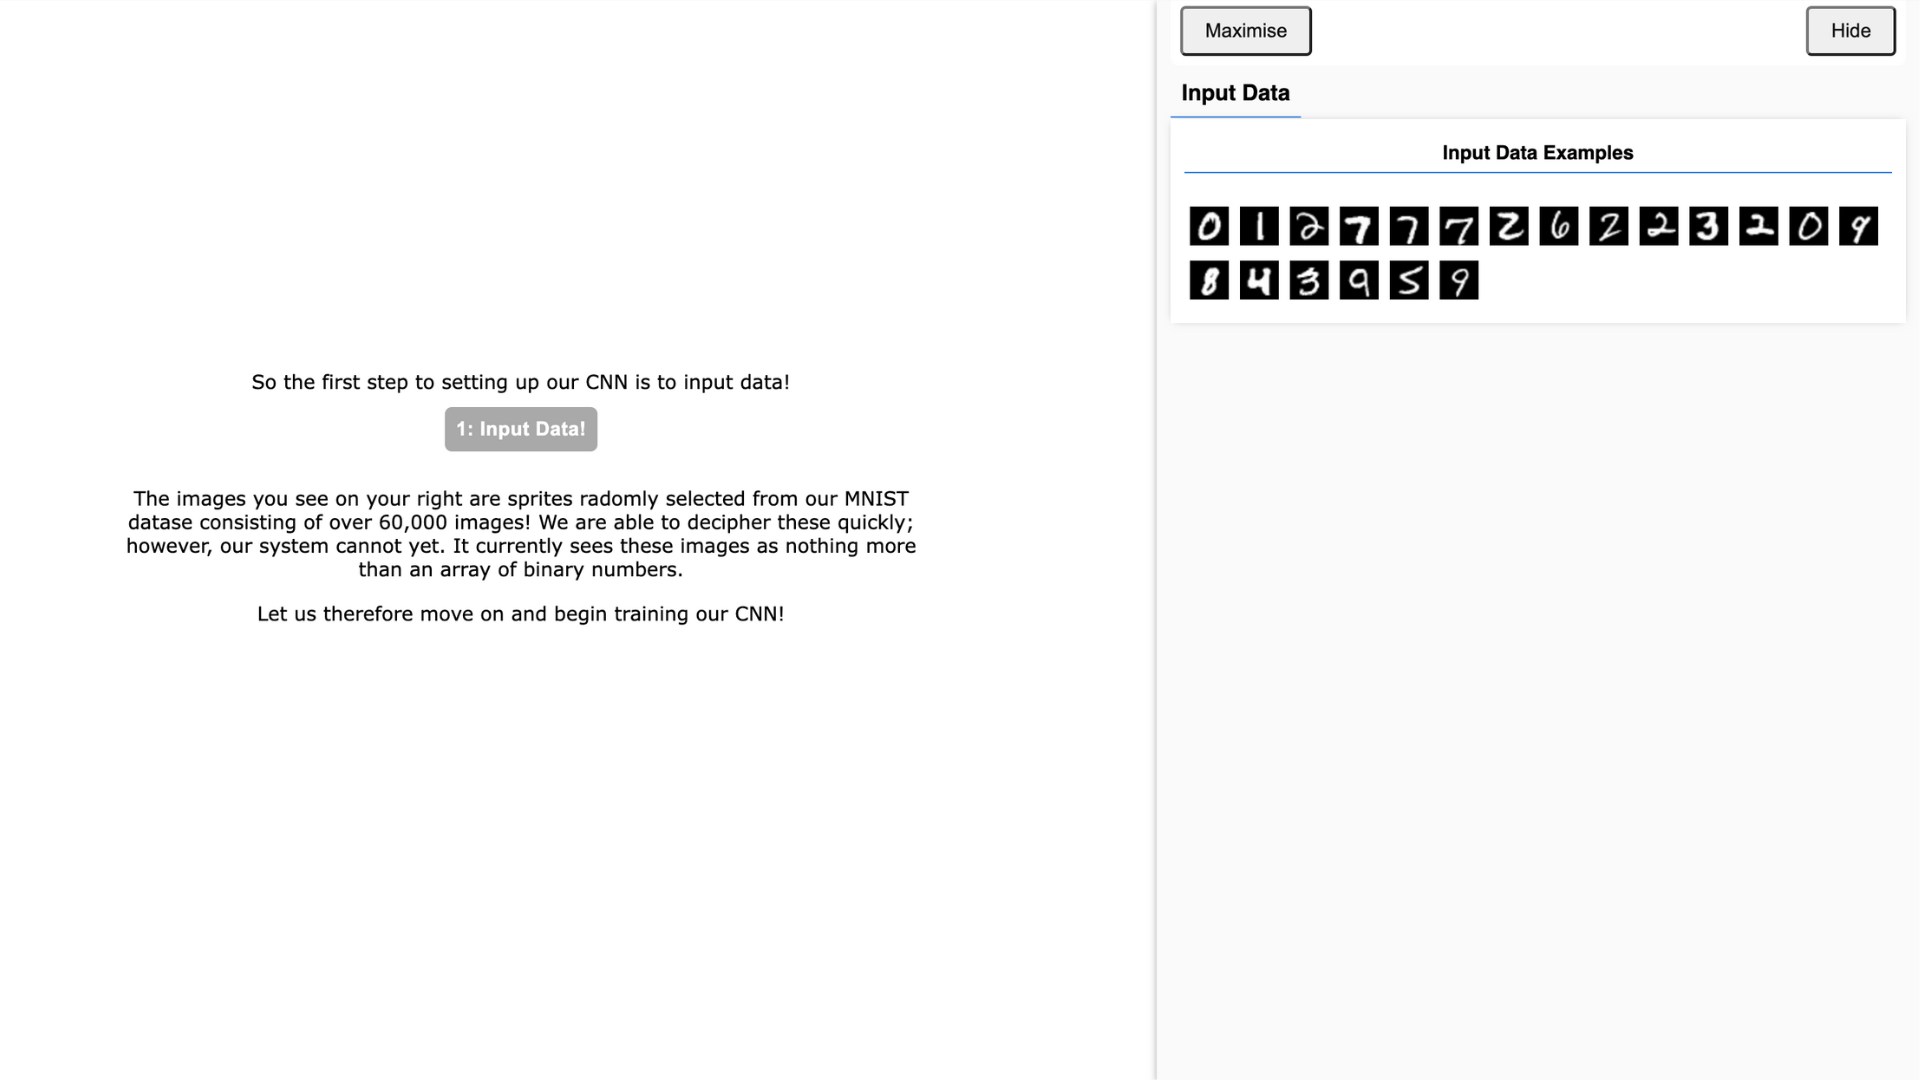
\includegraphics[width=0.4\textwidth]{./Images/FontSizeScreenShot.png}
\end{figure}

\subsection{Content Considerations}
The explorable explanation as it currently stands, strictly explains how a CNN works from a technical standpoint in revealing the usually invisible inside workings. However, the explorable explanation does not delve into the significance of understanding how explorable explanations work. Based on the our previously established definition of opacity, the explorable explanation does fulfill its role of bridging high-dimensionality of machine learning and human-scale reasoning; however, the website never explains complications that can occur within the mathematical processings of CNNs. The perceived superiority of black-box algorithms to interpretable algorithms still exists, never recognizing the importance and need for opacity as a way to break down that misconception. Though the explorable explanation displays that CNNs are not 100 percent accurate, it leaves it up to the viewer on how to interpret that bias. In this sense, the project could be better improved by explaining biases and breaking down why certain biases exist, how it affects systems in the real world, and how it can be (or is being) addressed. 


A large reason bias is not as addressed in this explorable explanation is due to the content referenced. In this explorable explanation, I purposely chose a simple example of the MNIST data to lower the bar of entry in learning about CNNs. However, by providing a simple, non-consequencial example lessens the stake of biases in ways CNNs are currently employed. As such, the best way to address this topic would to add on a section at the end, applying the CNN to a different more complicated data set like recognizing if something is a person or not. This could be applied to automated driving--if the CNN recognizes the images before it as a person, the car will stop, if not, it continues driving. However, if the car does not correctly identify a person as a person, it could result in a fatal crash. This allows for users to then apply what they have learned with the MNIST example of how a CNN technically works to a more complex and consequential example. This not only addresses the issue of bias but also brings the highest cognitive dimension up a level from understanding to applying. \cite{cognitiveDimension}

\appendix
\section{Replication Instructions}
In order to replicate the project, revisit the method section as it is written in chronological order of how the project is completed. The following list contains all software that is used: 
\begin{itemize}
    \item Figma for designing/prototyping
    \item Visual Studio Code for coding
\end{itemize}
The following languages are used in Visual Studio Code to implement the explorable explanation: 
\begin{itemize}
    \item HTML (HyperText Markup Language)
    \item Javascript
    \item CSS (Cascading Style Sheet)
\end{itemize}
The only library used in Javascript is \textbf{TensorFlow.js} to train and deploy a CNN model. 
For a tutorial on how to train and deploy an image categorization CNN program visit \href{https://www.tensorflow.org/js/tutorials/training/handwritten_digit_cnn}{www.tensorflow.org}.

\section{Code Architecture Overview}
As a UX/UI project, the code architecture of my project revolves around building a website. As such, the code in and of itself is not novel; however, for the sake of replication this section will go over the file architecture in which the code is sorted. The final explorable explanation consists of five files, excluding a folder for images and json files. They include the following:
\begin{itemize}
    \item \verb|index.html| : Contents of the frontend.
    \item \verb|index.css| : Cascading style script to design and format elements from the frontend
    \item \verb|script.js|: Backend for CNN code implementing TensorFlow.js
    \item \verb|data.js| : Backend processing of MNIST dataset 
    \item \verb|buttons.js| : Javascript for button functions
\end{itemize}

\printbibliography

\end{document}
